
% Chapter Template

\chapter{Estado del arte} % Main chapter title

\label{Chapter3} % Change X to a consecutive number; for referencing this chapter elsewhere, use \ref{ChapterX}

\section{HTCondor}
HTCondor es un sistema de gestión de carga de trabajo especializado para pruebas de ejecución de cálculo intensivo. Al igual que otros sistemas que hacen uso del batch con todas las funciones, HTCondor ofrece un mecanismo para trabajos en cola,  una política de planificación, un esquema de prioridades, el seguimiento de los recursos y la gestión de recursos. Los usuarios envían trabajos ya sea en serie o paralelos a HTCondor, HTCondor los coloca en una cola, decide cuándo y dónde ejecutar los trabajos en base a una política, monitorea cuidadosamente su progreso, y en última instancia, informa al usuario sobre la terminación.

Una de las tantas característica de HTCondor es que puede ser usado para administrar clusters conformados por nodos de computo dedicado. Aun así, también tiene la capacidad de configurarse para utilizar solamente nodos de computo no dedicados, de tal forma que emplea mecanismos para aprovechar los tiempos ociosos de la CPU siempre y cuando estos no presenten eventos en el mouse o teclado, por ejemplo, presionar alguna tecla. 

En el caso que un nodo no dedicado ( previamente se encuentre disponible u ocioso ) esté ejecutando alguna tarea enviada por HTCondor y algún usuario de dicho nodo realice algún evento en el teclado o mouse, HTCondor está en la capacidad de detectar este evento y parar la tarea en dicho nodo y reenviarla a otro nodo que sí se encuentre en estado ocioso o disponible (checkpoint). Otra característica muy importante y que lo convierte en una herramienta con una gran ventaja en comparación con otros gestores de trabajos, es que tiene un diseño limpio que simplifica el envío de trabajo de los usuarios por medio del mecanismo ClassAds (siglas en inglés de Classified Advertisements), el cual permite a los usuarios pedir recursos necesarios y deseados para ejecutar los trabajos.

Para hacer uso de esta herramienta, se debe contar con tres elementos claves, que son un nodo maestro (\textbf{Master}), uno o varios nodos donde ejecutar los trabajos (\textbf{Workers}) y un \textbf{universo de ejecución}.

\begin{itemize}
\item \textbf{Nodo maestro (Master)}: es el encargado de administrar y coordinar las tareas que van a ser ejecutadas en el cluster. Esto quiere decir, que es capaz de determinar cuáles nodos esclavos se encuentran disponibles o cuales son ideales para ejecutar una tarea. Por otra parte, este nodo también permite al usuario el acceso al cluster, por consiguiente, por cada grupo o entorno HTCondor(pool) debe existir únicamente un solo nodo master. Es de importancia resaltar, que este nodo también puede hacer el rol de worker y submit. A este nodo también se le conoce como Central Manager.
\item \textbf{Nodo trabajador (Worker)}:este tipo de nodo es el que está en capacidad de recibir y ejecutar las tareas enviadas por el nodo submit.
\item \textbf{universo de ejecución}: en HTCondor un universo es un entorno de ejecución el cual depende del tipo de aplicación que se desea ejecutar. Los universos son: standard, el cual provee confiabilidad y migración de las tareas por medio del mecanismo de checkpoint, para que un programa pueda ser enviado por medio de este universo, ha debido ser compilado con las librerías de HTCondor. vanilla, es el universo por defecto si no se especifica, aunque el administrador puede configurar HTCondor para que otro universo lo sea, es el menos restrictivo con los programas que se puedan enviar, ya que acepta cualquier programa escrito en cualquier lenguaje de programación, su desventaja es que no permite el mecanismo de checkpoint. El universo grid permite a los usuarios enviar trabajos usando la interfaz de HTCondor, estos trabajos son enviados para ser ejecutados sobre recursos que se encuentren en una grid. El universo java permite enviar trabajos escritos en lenguaje, el universo parallel es para enviar programas que requieran múltiples máquinas(nodos esclavos) para ejecutar un solo trabajo o aplicación paralela, para utilizarlo se debe hacer uso del estándar MPI ( siglas en ingles de Message Passing Interface ).

\end{itemize}

\section{Planta Física Universidad Tecnológica de Bolívar}

Distribución de la estructura física de los servidores con los que cuenta actualmente la Universidad Tecnológica de Bolívar
\begin{figure}[h]
\centering
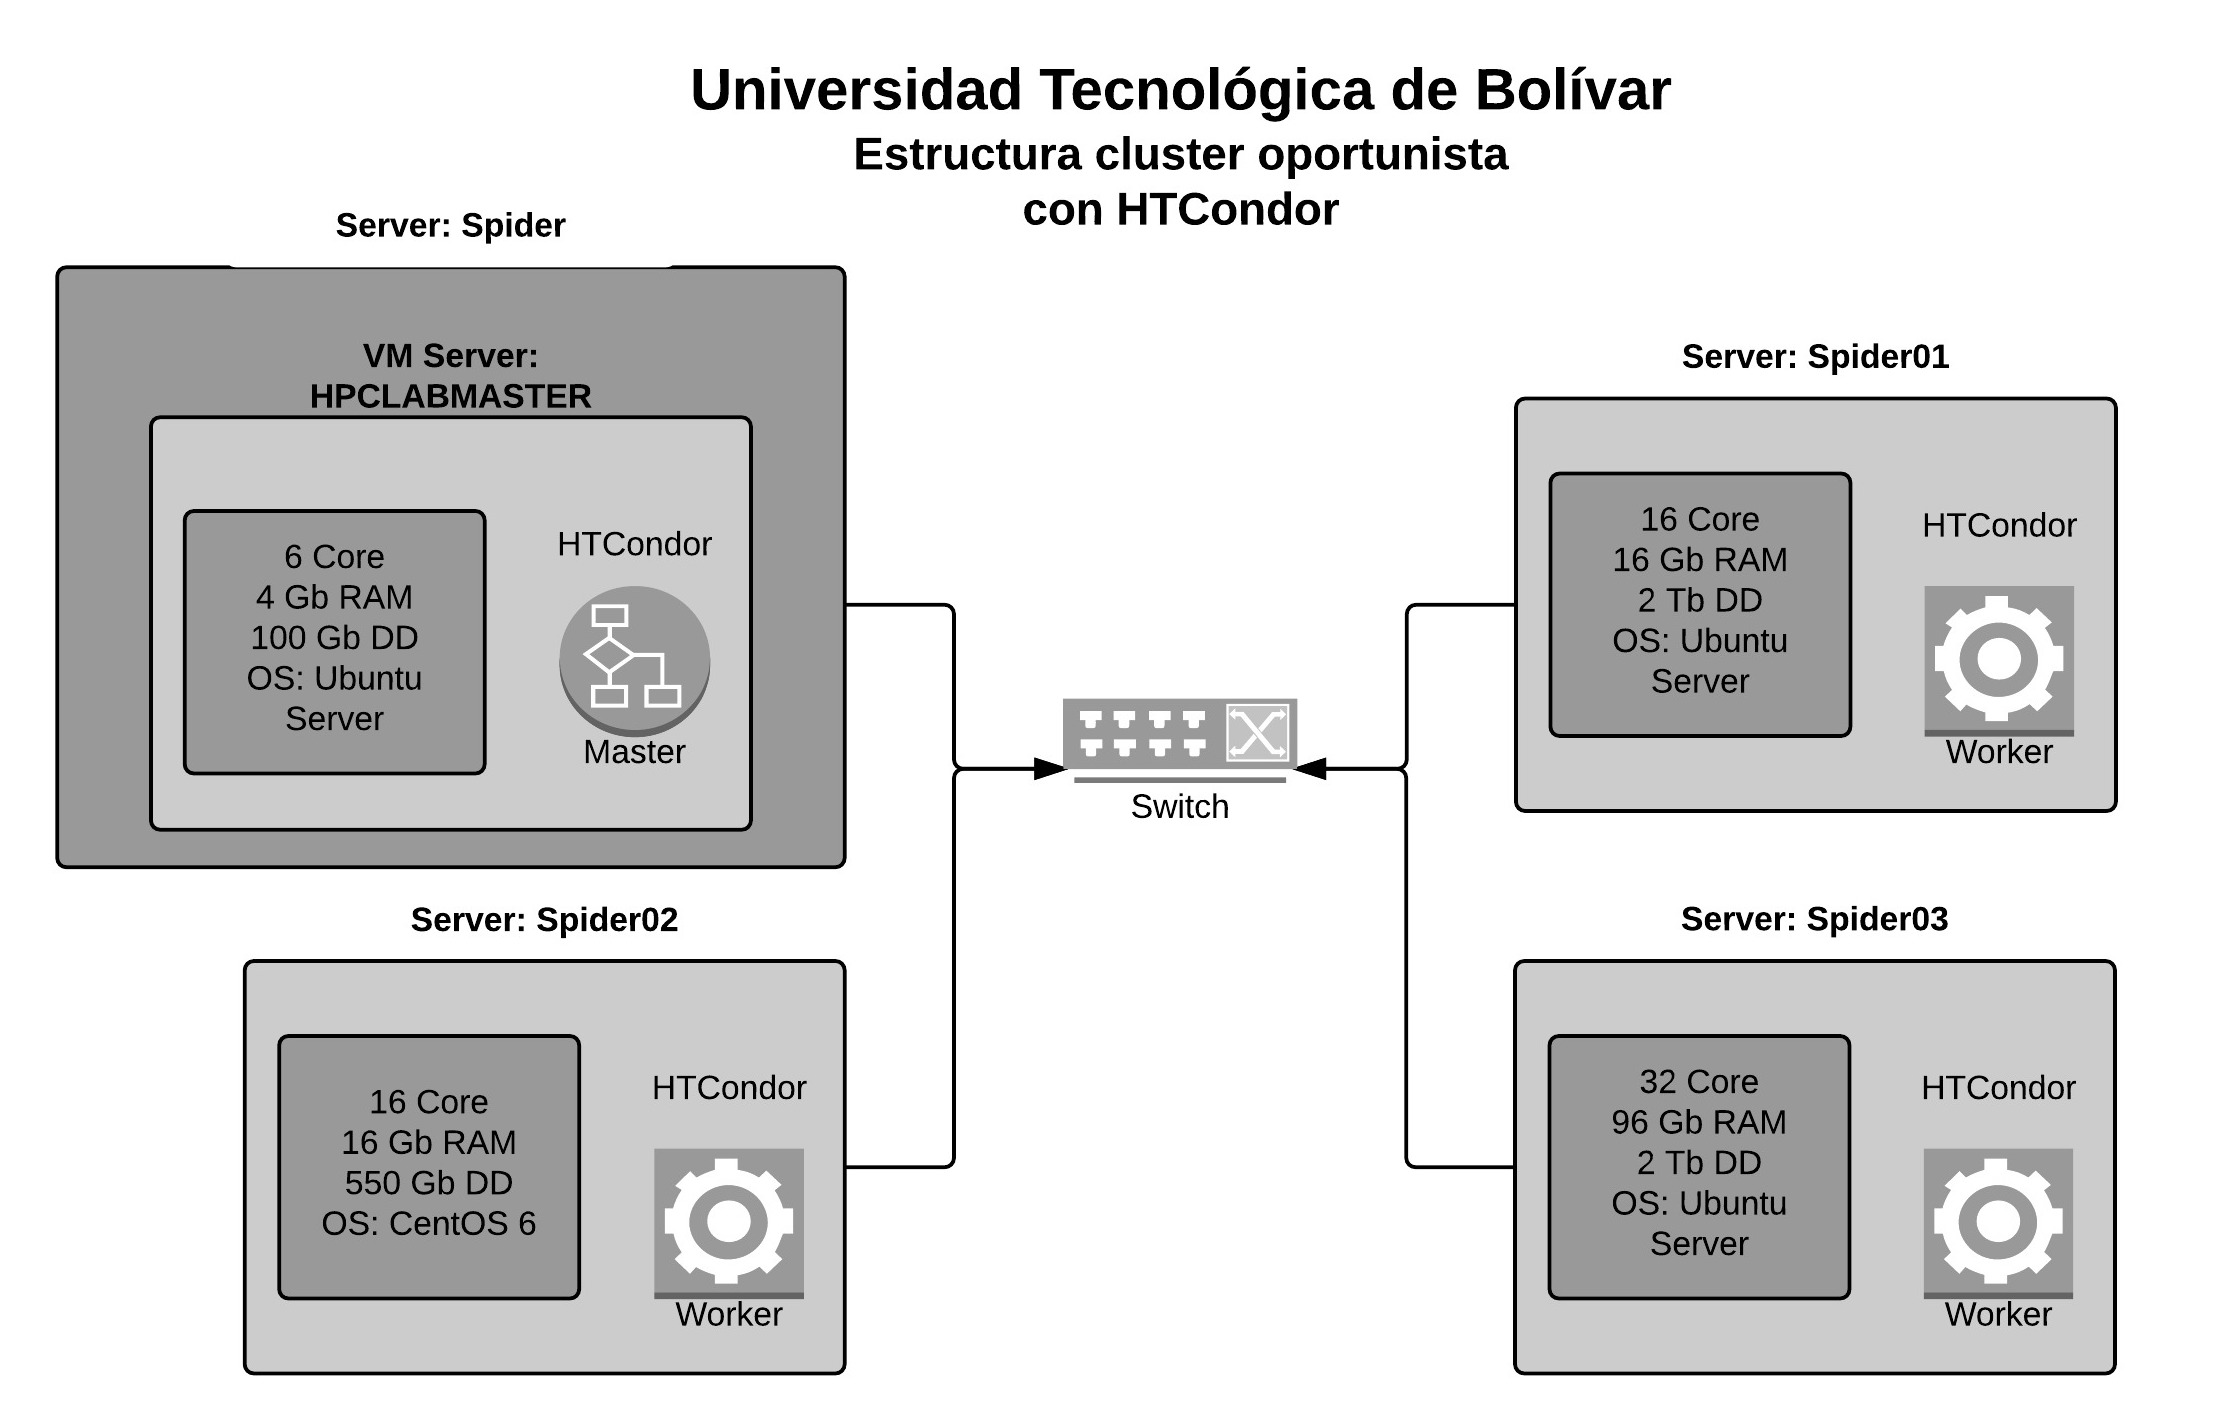
\includegraphics[width=0.95\textwidth]{images/spidercluster.jpeg}
\decoRule
\caption{Estructura HTCondor en la UTB}
\label{fig:UTB_Condor}
\end{figure}
\FloatBarrier

El nodo maestro es una máquina virtual instalada en el servidor físico \mbox{\textbf{Spider}}, esta máquina virtual cuenta con 6 procesadores, 4Gb RAM y 100Gb de espacio en disco para almacenamiento.

\begin{figure}[h]
\centering
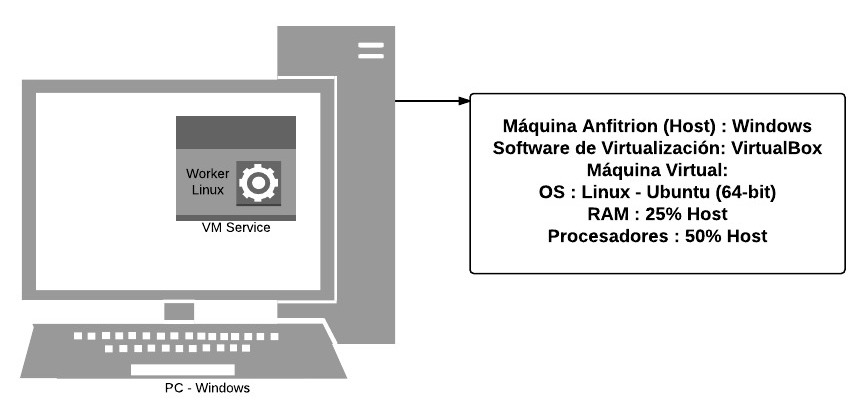
\includegraphics[width=0.95\textwidth]{images/workernode.jpeg}
\decoRule
\caption{Estructura HTCondor en Nodo Windows}
\label{fig:UTB_Condor}
\end{figure}
\FloatBarrier

Ademas de ello cuenta con 6 salones laboratorios que tienen 30 estaciones de trabajo con sistema operativo Windows que son el foco donde se \mbox{implementará} este trabajo.



